\chapter{Introduction}

\section{Pourquoi la vérification et la preuve de programmes?}

%Il est de fait complètement établi que la révolution informatique fut vue
L'informatique était vue comme la solution pour résoudre les problèmes de
fiabilité dans les domaines où toute défaillance 
opérationnelle peut conduire à des catastrophes. L'étymologie du mot {\em ordinateur}
est un bel exemple des espoirs que l'on a placés dans le domaine. Introduit par Jacques Perret
en 1955, il est issu du latin {\em ordinator} qui signifie celui qui met en ordre, qui règle
\footnote{\footnotesize Extrait de la définition d'{\em ordinator} dans le dictionnaire Gaffiot}.
Cette définition omet de préciser que si l'ordinateur sait résoudre des problèmes, c'est 
grâce à l'ordonnateur (plus communément appelé programmeur ou développeur). %dont il 
L'ordinateur exécute les directives (le programme) du programmeur susceptibles de résoudre
les problèmes auxquels la machine est assignée. 
Si la machine est incontestablement meilleure que toute personne humaine dans la répétition 
intensive de calcul, l'introduction de l'informatique déplace simplement le problème 
de la fiabilité: le programme est-il suffisamment bien conçu pour permettre à l'ordinateur
de toujours réussir dans sa tâche? 

Si l'on se concentre sur la tâche du programmeur, celle-ci peut se résumer essentiellement
en deux étapes. Analyser le problème, puis si une méthode de résolution (au sens algorithmique du terme) existe,
la traduire en une spécification opérationnelle, le programme. Le {\em bug}\footnote{\footnotesize
  La terminologie française exacte est {\em bogue}} intervient lorsqu'une faute 
de raisonnement conduit à une spécification erronée ou incomplète : conduisant l'ordinateur 
dans des comportements inattendus qui constituent les manifestations cliniques du bug.
Plus le problème à résoudre est complexe, plus il y a de chance de commettre une faute 
de conception conduisant à un bug lors de l'exécution du programme. 
De l'analyse du problème on peut aussi aboutir à une spécification dénotationnelle et formalisée à l'aide d'outils mathématiques.
Cette spécification "haut-niveau" est univoque et constituée de définitions et de propriétés simples:
la spécification dénotationnelle est souvent plus facile à comprendre que la spécification opérationnelle puisque 
débarrassée des aspects calculatoires.
On oblige les programmeurs à commenter leur code source pour une bonne raison. La spécification opérationnelle
étant peu compréhensible, il est nécessaire de donner au moins une spécification informelle pour qu'une personne autre
que le programmeur soit capable de comprendre le programme.

Une partie de la science informatique a pour unique but de rendre la conception de programmes
plus sûre. L'idée sous-jacente pour mener à bien cet objectif est de rapprocher 
la spécification opérationnelle d'une spécification dénotationnelle,
pour simplifier le plus possible la phase de conception que doit effectuer le programmeur.
C'est en partie le but recherché par les langages de programmation.
Ils se basent sur des logiques ou des paradigmes particuliers, qui peuvent se révéler plus ou moins
adaptés à certains types de problèmes algorithmiques. Au milieu des années 90, on recensait plus 
de 2000 langages~\cite{DOWEK-LANG}. Un langage de programmation repose 
sur un générateur (compilateur) ou un interprète (machine virtuelle) assurant la traduction automatique
du code source "haut-niveau" vers le code machine "bas-niveau".

Idéalement, on pourrait imaginer que la formalisation dénotationnelle soit suffisante
pour exprimer le programme à réaliser: par exemple un programme de tri est un programme
qui, à partir d'une liste, fournit une permutation de cette liste où les éléments sont
ordonnés. Cela reviendrait à ne donner que des définitions extensionnelles des programmes~\cite{DOWEK-LANG}.
Cependant, du point de vue du programmeur celles-ci ne sont pas assez expressives. 
Par exemple, alors qu'ils produisent le même résultat le tri à bulles et le tri rapide ne sont pas équivalents
d'un point de vue opérationnel.
% mais pas assez expressif: il est impensable pour tout bon programmeur de considérer comme équivalent le tri-rapide
% et le tri-à-bulles alors qu'ils produisent le même résultat une liste d'éléments triés.
A la place, on préfère utiliser une spécification dénotationnelle et vérifier à posteriori
que le programme est correct vis-à-vis de cette spécification. 
Un exemple commun est le système de types dans les langages de programmation. 
Lorsque le programme est correct,\textit{i.e.} si la vérification des types réussit,
on a l'assurance que le programme est sûr: 
les manipulations et les calculs qu'il effectue sont toujours réalisés sur des données
bien interprétées. Il n'y a pas de risque de confusion entre un entier et une adresse mémoire
(Un chou est un chou!~\cite{ASTERIX}).
Dans le cas des systèmes de types, la spécification dénotationnelle est facile à construire
car il s'agit d'annotations intégrées directement au langage. Pour exprimer
des propriétés plus fortes, on a souvent besoin d'un langage de spécification beaucoup
plus évolué qui prend place à côté du code source en commentaire (ex: JML pour Java) ou 
dans un fichier séparé.

Il est aussi possible de se passer d'une partie des  annotations dans certains langages modernes,
celles-ci pouvant être inférées automatiquement pour certaines vérifications.
Dans ce cas, une analyse automatique et statique (sans exécution) du programme
déduit automatiquement une spécification particulière, à partir de laquelle s'effectue la 
vérification. Certains types de propriétés peuvent être vérifiés de manière
complètement automatique.  Parmi les domaines qui fournissent des outils à l'analyse statique,
on peut citer les analyses utilisant la génération de contraintes sur les variables du programme, 
la théorie de l'interprétation abstraite~\cite{CousotC-POPL77} ou le model-checking~\cite{MC-Book}.
L'interprétation abstraite génère automatiquement une abstraction de l'ensemble des comportements possibles
du programme analysé pour des domaines particuliers. Le model-checking fournit aussi des outils d'analyses 
entièrement automatiques pour la vérification de propriétés temporelles mais suppose qu'une spécification opérationnelle
"haut-niveau" mais correcte du programme est fournie. 
Enfin, lorsque les propriétés sont trop difficiles à prouver automatiquement, on peut
faire appel à des assistants de preuves~\cite{Coq, Isa, Agda} qui permettent de construire interactivement 
des preuves correctes de programmes: le langage de l'assistant est assez expressif pour
exprimer le programme et ses propriétés. Des outils comme KeY~\cite{KEY} pour Java, Frama-C~\cite{FRAMAC} pour le C
génèrent à partir d'une spécification formelle et du code source d'un programme
des obligations de preuves que l'utilisateur doit prouver (soit à la main soit automatiquement)
afin d'assurer la correction du programme vis-à-vis de la spécification.

\section{La réécriture pour modéliser les programmes}

La réécriture est un modèle de calcul communément utilisé en informatique.
Elle formalise le calcul par des règles de transformation syntaxique pour des objets tels
que des mots ou des termes par exemple. 
Une règle de réécriture est un objet de la forme $l \rw r$.
La règle de réécriture s'applique à un objet $t$ si celui-ci contient une instance compatible
avec $l$ le membre gauche de la règle. Lorsque l'application est possible, on dit que $t$ se réécrit en un nouvel objet $t'$
que l'on obtient en remplaçant l'instance du membre gauche $l$ par l'instance du membre droit $r$ correspondante.
Mais on s'intéresse plus particulièrement à la réécriture de termes.
Un exemple courant est la définition des opérations élémentaires sur les entiers naturels suivant l'axiomatisation
de Peano: les termes sont alors définis par les opérateurs usuels $\_\ *\ \_$, $\_\ +\ \_$ sur les entiers naturels
représentés par $0 \in \Nat$ et $Sn \in \Nat$ qui représentent le successeur de l'entier $n \in \Nat$. Ainsi $SSS 0$
que l'on peut abréger par la notation $S^3 0$ correspond à l'entier naturel que l'on note plus volontiers $3$.
On peut définir la calcul de l'addition et de la multiplication, chacune par deux règles de la façon suivante :
\[
\textrm{ Addition :}\left\{
\begin{array}{l}
  0 + x \rw x\\
  S x + y \rw x + S y
\end{array}\right.
\quad
\textrm{ Multiplication :}\left\{
\begin{array}{l}
  0 * x \rw 0\\
  S x + y \rw (x * y) + x
\end{array}\right.
\]
Les variables $x$ et $y$ peuvent être remplacées par n'importe quel terme, pour constituer l'instance du membre gauche
d'une règle de réécriture. Par exemple le terme $t = SS0 + SS0$ constitue une instance du membre gauche de la règle
$S x + y \rw x + S y$ en posant $x = S0$ et $y = SS0$: on peut donc réécrire $t$ en $t' = S0 + SSS0$. 
A contrario, $t$ et $t'$ ne contiennent pas d'instance pour appliquer la règle $0 + x \rw x$.
En répétant successivement les étapes de réécriture, on obtient la chaîne de réécriture suivante:
\[ SS0 + SS0 \lrw S0 + SSS0 \lrw 0 + SSSS0 \lrw SSSS0 \]
La transformation syntaxique de $SS0 + SS0$ en $SSSS0$ correspond au résultat attendu pour l'opération $2$ "plus" $2$ 
qui est égal à $4$.

\newcommand{\fib}{\mathit{fib}}

L'expressivité des systèmes de réécriture permet de modéliser plus que l'arithmétique. 
En particulier tout système calculatoire peut-être modélisé, dont les programmes informatiques
par exemple. En fait, certains langages de programmation comme \ocaml~\cite{OCAML} ou \tom~\cite{TOM}
intègrent nativement la réécriture. L'exemple suivant donne un codage de la
célèbre\footnote{\footnotesize au moins chez les mathématiciens et les cuniculiculteurs} fonction de Fibonacci.
On note par $\fib(n)$ le nombre de Fibonacci de rang $n$. En reprenant et complétant la formalisation des entiers
naturels précédente, on peut définir la fonction $\fib(n)$ de la manière suivante:
\[
\begin{array}{l}
  \left\{\begin{array}{l}
      0 \le y \rw true\\
      Sx \le Sy \rw x \le y\\
      Sx \le 0 \rw \false
    \end{array}\right.
  \hspace*{4cm}
  \left\{\begin{array}{l}
      x - 0 \rw x\\
      Sx - Sy \rw x - y\\
      0 - Sy \rw \bottom
    \end{array}\right.\\
  \\\\
  \left\{\begin{array}{l}
      \ifte(\true, x, y) \rw x\\
      \ifte(\false,x, y) \rw y
    \end{array}\right.\\\\
  \hspace*{1.2cm}\fib(x) \rw \ifte(x\le S0, S0, \fib(x - S0) + \fib (x - SS0))
\end{array}
\]

\section{Vérification de systèmes de réécriture}

On peut remarquer que la définition de la fonction utilise la définition de la soustraction qui n'est que partiellement
définie, ce que l'on symbolise ici par la réécriture en $\bottom$. On peut donc se demander si la fonction $\fib$ 
est correctement définie pour tout $n \in \Nat$, c'est à dire qu'elle ne produit jamais le terme
$\fib(\bottom)$ correspondant simplement à un plantage du programme.

Une manière de vérifier que le système de réécriture n'engendre pas le terme $\fib(\bottom)$ est de générer tous les 
termes que peut produire le système de réécriture. 
Pour cela on peut décider de représenter l'ensemble des termes initiaux $\fib(n)$, correspondant à l'ensemble des valeurs 
puis de calculer l'ensemble des termes que l'on peut obtenir, qui correspondent finalement à l'ensemble des valeurs
possibles que peut prendre le programme. La technique consiste à compléter itérativement l'ensemble $I$, 
par les nouvelles valeurs que peut prendre la fonction jusqu'à ce l'ensemble soit saturé. On note cet ensemble $\R^*(I)$
c'est à dire l'ensemble des termes atteignables par réécriture des termes initiaux.

\begin{figure}[ht!]
  \centering
  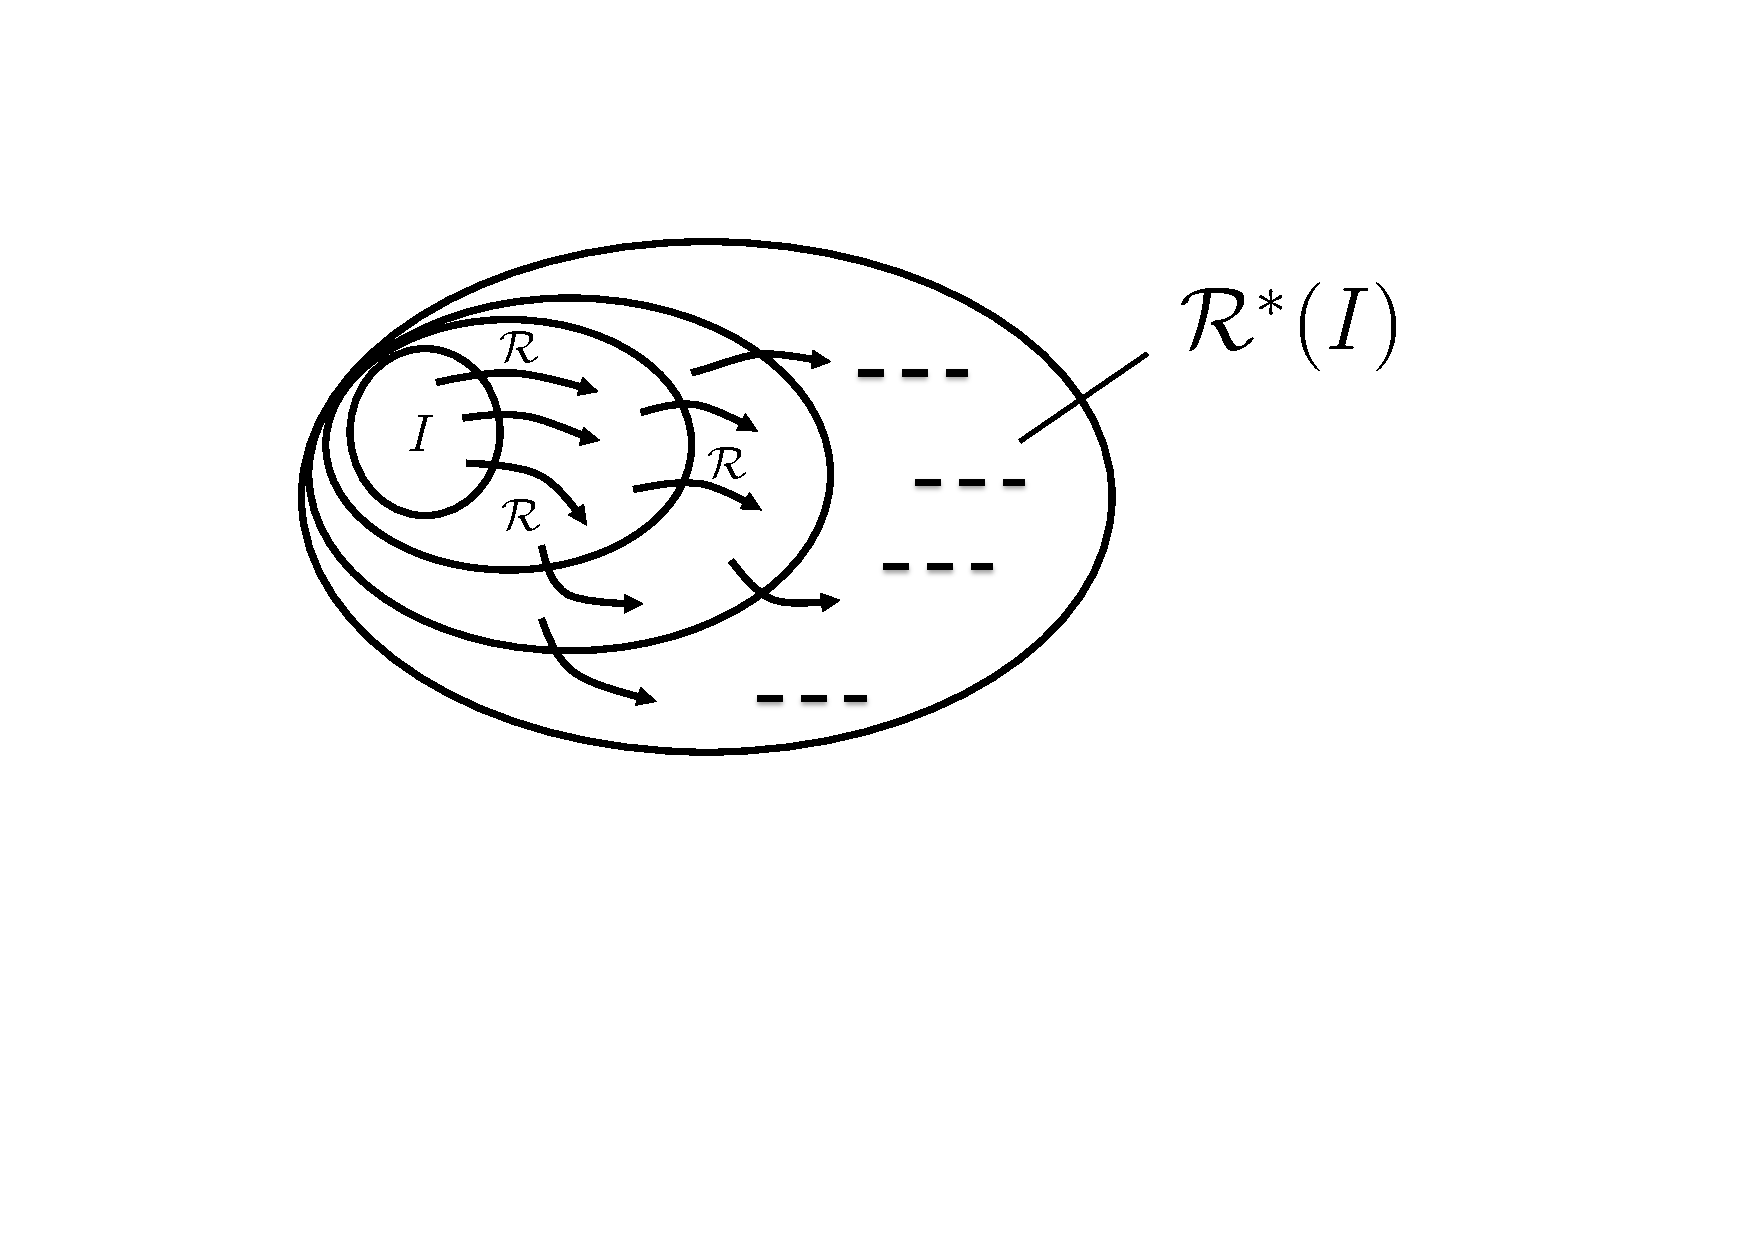
\includegraphics[width=12cm]{1_intro/exact}
\end{figure}

En supposant que l'on sait calculer $\R^*(I)$, on est alors à même de vérifier que le terme $\fib(\bottom)$
n'est jamais produit. C'est ce que l'on appelle communément le problème d'atteignabilité.

Mais plusieurs problèmes doivent être résolus pour être capable de
calculer $\R^*(I)$.  L'ensemble des termes initiaux peut être infini,
comme c'est d'ailleurs le cas pour la fonction de Fibonacci.  Il faut
donc fournir une représentation finie d'un ensemble infini.  Les
automates d'arbres sont une approche tout à fait indiquée pour
résoudre ce problème sur les termes.  Cependant, tout ensemble de
termes n'est pas représentable par un automate d'arbres.  Et c'est
souvent le cas de l'ensemble des états accessibles d'un programme, et
des termes atteignables d'un système de réécriture qui le
modélise. On peut en déduire qu'il n'existe pas toujours d'automate
d'arbres capable de représenter l'ensemble des termes
atteignables. En fait, de manière plus générale, il n'est pas possible
de calculer (et de représenter) l'ensemble des termes atteignables
pour un système de réécriture donné.  Par contre, il est possible d'en
calculer une sur-approximation.  C'est l'objectif de la complétion
d'automates d'arbres : compléter le langage\footnote{\footnotesize
  l'ensemble des termes représenté par l'automate} d'un automate
d'arbres en ajoutant successivement les termes atteignables.  C'est un
semi-algorithme introduit par Th.~Genet~\cite{Genet-RTA98}, qui
calcule un automate $\aapprox$ caractérisant une sur-approximation
d'un ensemble $\R^*(I)$.  Lorsqu'il n'est plus possible de compléter
l'automate, ce dernier est clos par réécriture, c'est à dire qu'il
contient tous les termes atteignables.  L'approximation est paramétrée
par $E$ un ensemble d'égalités (ou équations) qui définissent des
classes d'équivalence qui permettent des raccourcis syntaxiques.  Par
exemple, on peut définir les équations $x + y = y + x$ pour définir la
commutativité de l'addition ou $Sx = SSx$ pour considérer tout entier
(sauf $0$) équivalent à son successeur: on partitionne alors les
entiers en deux classes $\dot{0}$ et $\dot{1}$.  La complétion est un
semi-algorithme, car si l'ensemble d'équations ne construit pas des
classes d'équivalence assez fortes, alors le calcul diverge.

\begin{figure}[ht!]
  \centering
  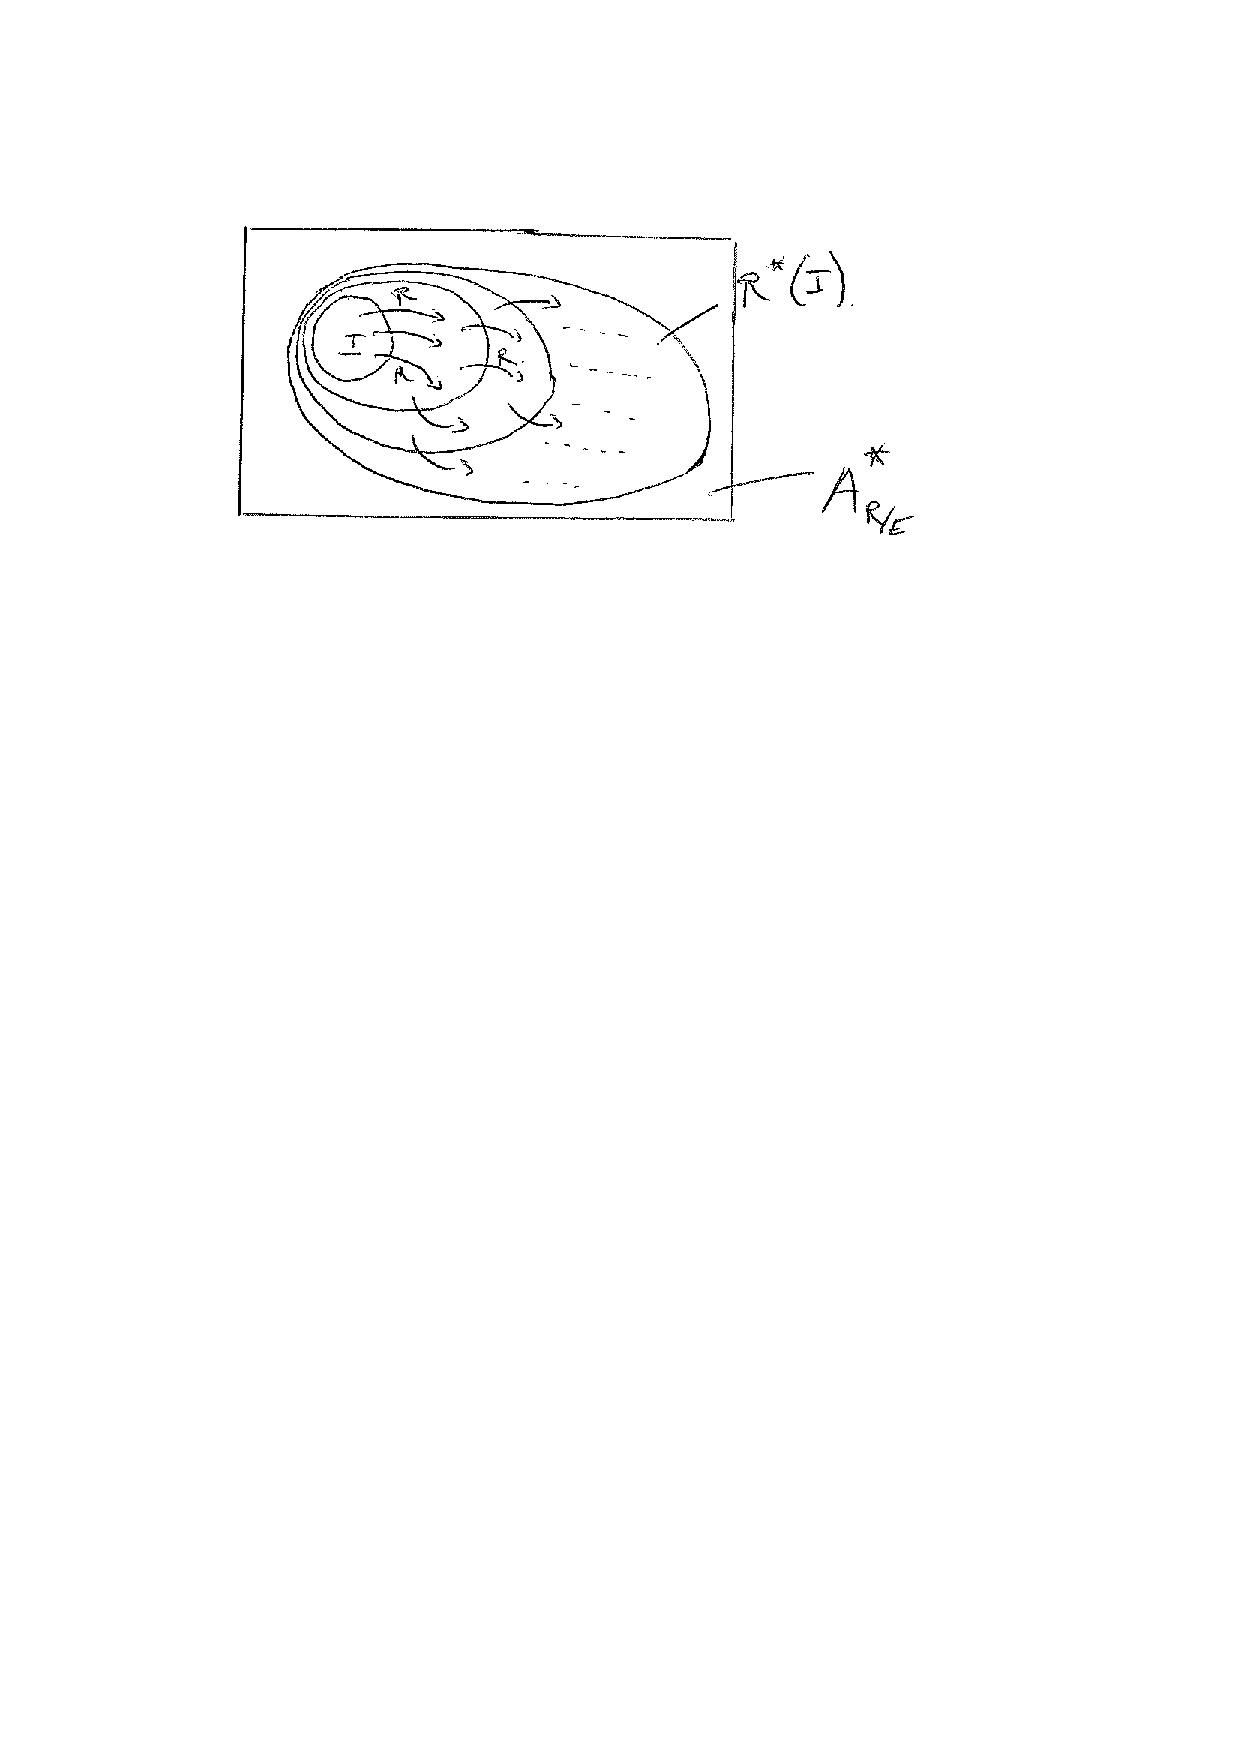
\includegraphics[width=12cm]{1_intro/approx}
\end{figure}

Du point de vue du problème d'atteignabilité, calculer une sur-approximation reste correct: en effet, si le terme $\fib(\bottom)$ 
n'est pas dans la sur-approximation de $\desc(I)$ alors il n'est clairement pas dans $\desc(I)$
non plus. Par contre, si la vérification échoue on ne peut rien dire.
L'outil \timbuk~\cite{timbuk} implémente l'algorithme de complétion et permet de vérifier des propriétés
de sûreté sous forme de problème d'atteignabilité. Il est utilisé principalement dans la
vérification des protocoles cryptographiques. Il se base sur une spécification symbolique 
et opérationnelle du système à vérifier, c'est à dire un système de réécriture où les termes sont les états possibles
du protocole, et les règles de réécriture modélisent les transitions du protocole.
Il fonctionne suivant le principe illustré ci-dessus.
Plus récemment, il a été montré qu'il est possible de modéliser un sous-ensemble important du ByteCode Java
par un système de règles de réécriture~\cite{BoichutGJL-RTA07}. Les termes du systèmes représentent les états
de la machine virtuelle Java, et les règles de réécriture la sémantique de Java. L'outil Copster~\cite{Copster} 
génère à partir d'un fichier \texttt{.class} le système de réécriture: l'exécution du système de réécriture 
correspond exactement à l'exécution du programme Java. 



\section{Présentation des Contributions de cette thèse}
Les contributions de cette thèse trouvent leur place dans le cadre de vérification de programmes Java
compilés en systèmes de réécriture et dont l'analyse se base sur la complétion d'automates d'arbres.
La complétion a pour ambition de proposer une technique intermédiaire entre la preuve de programme
entièrement réalisée à la main, et les outils d'analyse statique.
Ces derniers, bien qu'ils soient complètement automatiques, présentent le défaut de ne traiter que 
certains types de propriétés reposant sur une théorie qui est décidable, comme l'interprétation abstraite et le model-checking.
La complétion permet de définir un cadre de vérification semi-automatique grâce à une abstraction
régulière paramétrable en fonction de l'analyse et des propriétés à vérifier.
La seule intervention dans le processus d'analyse reste la construction de l'ensemble d'équations
qui peuvent être générées automatiquement ou fournies directement à la main. Dans ce dernier cas, 
le degré d'expertise requis est toujours moins important que celui nécessaire à la preuve de programme
entièrement manuelle. D'autre part, l'approximation calculée est toujours correcte, quelle que soit l'abstraction choisie.
%ce qui n'a pas besoin d'être démontré pour chaque nouveau domaine. 
% A l'opposé, on trouve les assistants de preuves permettant
% la spécification et la construction de preuves de programmes à la main. Cette approche a le défaut
% d'être extrêmement coûteuse en temps et requiert un important niveau d'expertise dans la preuve de programme en général. 
% Les analyses basées sur la complétion d'automates d'arbres tente de s'intercaler entre ces deux univers
% en tant qu'outil de vérification semi-automatique. 
% En effet, l'analyse est basée sur un calcul sur-approchant tous les comportements du systèmes, 
% dont l'approximation est facilement paramétrable.
Les travaux de cette thèse ont pris place dans le projet de l'ANR Ravaj~\cite{RAVAJ}.
Les objectifs du projet portaient notamment sur l'adaptation de la complétion à l'analyse d'applications Java
et la certification des analyses effectuées. 
% Plusieurs objectifs ont été soulevés dans ce projet comme l'adaptation de la technique de complétion
% afin de réaliser ce type d'analyse d'une part, mais aussi l'aspect certification de l'analyse dans le
% but d'obtenir un degré de confiance élevé dans la technique proposée. 
En cours de projet, deux autres objectifs se sont dégagés comme le passage à l'échelle,
mais aussi le besoin d'étendre les propriétés vérifiables à la logique temporelle.
% L'outil \timbuk\ %qui est l'implémentation initiale
% était initialement destiné à la vérification de protocoles cryptographiques. 
% Pour les protocoles, les systèmes de réécriture sont de petite taille et la définition d'abstraction 
% réclame une expertise pointue mais réaliste.
Dans le cas des programmes en ByteCode Java, la taille des systèmes de réécriture est trop importante
pour espérer construire à la main une bonne abstraction. La première contribution de cette thèse est de
proposer une technique de raffinement automatique d'approximation
afin de réduire l'expertise nécessaire à la définition des équations.
La deuxième contribution étend les propriétés vérifiables par la complétion aux propriétés temporelles.
Enfin la troisième contribution est de certifier les analyses effectuées.



\bigskip
\subsection*{Le raffinement automatique} 
L'objectif du chapitre~3 de cette thèse est de montrer comment étendre la complétion
aux techniques de raffinement automatique de l'abstraction. Fournir une abstraction permettant à la complétion
de terminer est faisable même pour les programmes Java. Le problème est de fournir une abstraction qui soit assez
fine pour vérifier la propriété attendue, tout en assurant la terminaison. Sous ces contraintes, quel que soit
le niveau d'expertise, il est à peu près impossible de définir à la main la bonne abstraction. Le raffinement automatique
de l'abstraction permet de simplifier cette tâche: on peut alors définir une abstraction peu précise mais qui assure
la terminaison du calcul, l'abstraction étant affaiblie automatiquement lorsque c'est nécessaire.
La contribution de ce chapitre est double. Tout d'abord, elle offre à la complétion la possibilité de
construire des contre-exemples. Cette fonctionnalité, bien qu'indispensable, était absente et difficile à mettre
en place dans le formalisme d'origine. Ensuite, on propose un algorithme de raffinement, non pas basé 
sur une tabulation des étapes de calculs et sur des calculs arrières qui peuvent s'avérer coûteux, mais sur un élagage 
original de l'automate construit. 
% On propose d'étendre la complétion d'automates d'arbres afin de détecter les cas où l'abstraction se
% trouve justement trop grossière, ainsi qu'une technique de raffinement basée sur l'élagage de l'automate.
% L'apport est double car la procédure de raffinement permet une détection systématique lorsque le programme viole
% la propriété attendue.

Ce chapitre est actuellement en cours de soumission.% à la conférence~TACAS~2011.

\bigskip
% La seconde contribution de cette thèse s'intéresse à étendre le type de propriétés prouvables par la complétion.
\subsection*{La vérification comportementale}
Le chapitre~4 montre comment la complétion d'automates d'arbres peut être utilisée afin de vérifier 
des propriétés temporelles sur le graphe d'appels des méthodes d'un programme Java. Il est difficile 
de montrer des propriétés avec une composante temporelle en se basant uniquement sur la vérification du
problème d'atteignabilité. Une propriété comme 
"{\em si l'utilisateur clique sur le bouton Non, alors la requête ne sera pas émise sur le réseau}" est un exemple
des propriétés que l'on souhaiterait prouver sur des programmes Java. Dans ce chapitre, on montre comment tirer partie
de l'information contenue dans l'automate. %La complétion construit des automates qui contiennent naturellement une abstraction de la relation de réécriture. 
Cette abstraction de la réécriture correspond à une abstraction 
de l'exécution du programme qui induit notamment la construction explicite du graphe d'appels des méthodes Java.
On montre comment extraire cette information de l'automate complété, et comment utiliser les techniques standard
de vérification issues du model-checking, ce qui permet de vérifier des propriétés en logique temporelle~LTL.

Les travaux du chapitres~4 ont été présentés lors du workshop~Rule'09~\cite{BoyerG-RULE09}.

\bigskip
\subsection*{La certification de la complétion}
Le chapitre~5 décrit les travaux réalisés dans l'assistant de preuves \coq\ pour certifier la
complétion d'automates d'arbres. L'outil \timbuk\ a été notablement optimisé, et par ailleurs, différentes implémentations 
ont vu le jour. Certaines de ces implémentations n'utilisent plus les automates d'arbres au niveau algorithmique mais uniquement
comme format d'entrée du problème et comme format de sortie pour le résultat. %n'utilisent plus les automates d'arbres que pour produire le résultat final.
Par conséquent, ces outils sont de plus en plus éloignés de la spécification originale
de l'algorithme. Les optimisations sont une source de bugs supplémentaires, généralement difficiles à repérer.
% Les bugs loin d'être absents sont souvent durs à identifier:
% les optimisations sont une source de bugs car elles peuvent introduire des cas particuliers qui peuvent être 
% difficiles à repérer à l'origine des bugs. 
D'autre part, les implémentations %récentes étant plus performantes, elles 
sont capables de traiter des problèmes de taille beaucoup plus importante. Comme le résultat est non vérifiable à la main,
il est difficile de se convaincre de sa correction. L'ensemble de ces constats a permis de conclure qu'il était nécessaire de
vérifier les résultats de ces outils, de manière à obtenir une preuve \coq\ de la validité des résultats. C'est le rôle que joue
le vérificateur certifié en \coq. A partir d'une spécification de la réécriture et des automates d'arbres en \coq, on formalise
la correction d'un automate point fixe par rapport au problème d'atteignabilité. On montre ensuite comment vérifier la propriété
en \coq, ce qui définit le vérificateur. Ensuite, il est possible d'extraire puis de compiler un vérificateur 
conforme à la spécification \coq. Celui-ci permet de vérifier la validité de chaque résultat obtenu par un des outils
qui implémentent la complétion.

Le chapitre~5 a aussi fait l'objet d'une publication lors de la conférence IJCAR'08~\cite{BoyerGJ-IJCAR08}.

%En vérification 
%%% Local Variables: 
%%% mode: latex
%%% TeX-master: "../main"
%%% End: 
